% !TeX root = ../main.tex
% Add the above to each chapter to make compiling the PDF easier in some editors.

\section{Design Guidelines}
In this section, we explore the foundational principles guiding the Benchy Viewer's user interface. Rooted in Material Design, the application employs Material UI components for a clean and familiar look. The deliberate color scheme, restricted to black, white, and gray accents, promotes simplicity.

Moving on, we delve into the sidebar and the header, ensuring constant visibility and facilitating seamless navigation. The sidebar acts as a central hub, offering functionalities from page navigation to data import. The header contains crucial elements like the legend, eliminating the need for one in each visualization.

Finally, we examine the application's pages: Analytics Dashboard, Query Plan View, and Input File View. Each serves a distinct purpose, from analysing benchmark data to offering a minimalist view of raw imported data. 


\subsection{User Interface Design Styles}
\subsubsection{Material UI}

The Benchy Viewer's design is rooted in the principles of Material Design \parencite*{material-design}, emphasizing a sleek and consistent user interface that aligns with modern design standards.\\
To ensure a cohesive and user-centric design, the application makes extensive use of predefined components from Material UI \parencite*{mui}. In our application, this includes buttons, inputs, toggles, sliders, data grids, icons, drop-down menus, and tooltips.

The inclusion of Material Design components contributes to an interface that is both user-friendly and familiar. Users can easily navigate through these components, thanks to the standardized styling that Material UI provides.

Icons within the Benchy Viewer serve as visual cues, representing familiar symbols that aid users in quickly grasping the functions they perform. This visual clarity aligns with Material Design's emphasis on intuitive iconography.

Settings options, presented in drop-down menus and other interfaces, follow Material Design practices. The design prioritizes user intuition, allowing individuals to interact with the application seamlessly without relying on extensive textual explanations.

By aligning with Material Design principles, the Benchy Viewer achieves a design that not only meets aesthetic standards, but also prioritizes user understanding and interaction efficiency. The incorporation of familiar components enhances the overall usability and accessibility of the application.


\subsubsection{Styling Characteristics}

The Benchy Viewer embraces a deliberate color scheme aimed at providing a clean design. This is achieved through a restraint to specific base colors, limiting the palette to black, white, and a gray accent color, as depicted in Figure~\ref{fig:colors}. By adhering to this minimalist approach, the application exudes a sense of simplicity, ensuring a visually uncluttered interface.



\begin{figure}[h]
  \centering
  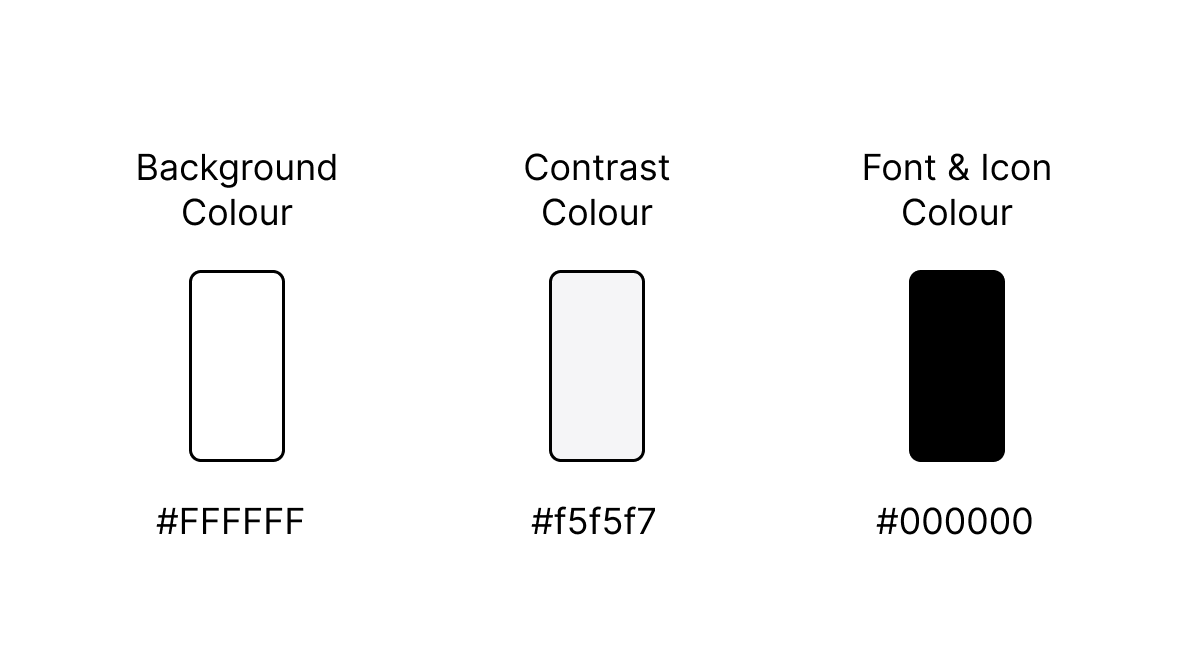
\includegraphics[width=0.4\linewidth]{figures/colors.png}
  \caption{Color palette of the user interface.}
  \label{fig:colors}
\end{figure}

While the overall design adheres to a subdued color palette, the visual elements within the application utilize a distinct color scheme, as illustrated in Figure~\ref{fig:colors-dbms}. This strategic approach guarantees that charts, plots, and other visual elements command attention, supporting users to focus on those data visualizations.

\begin{figure}[h]
  \centering
  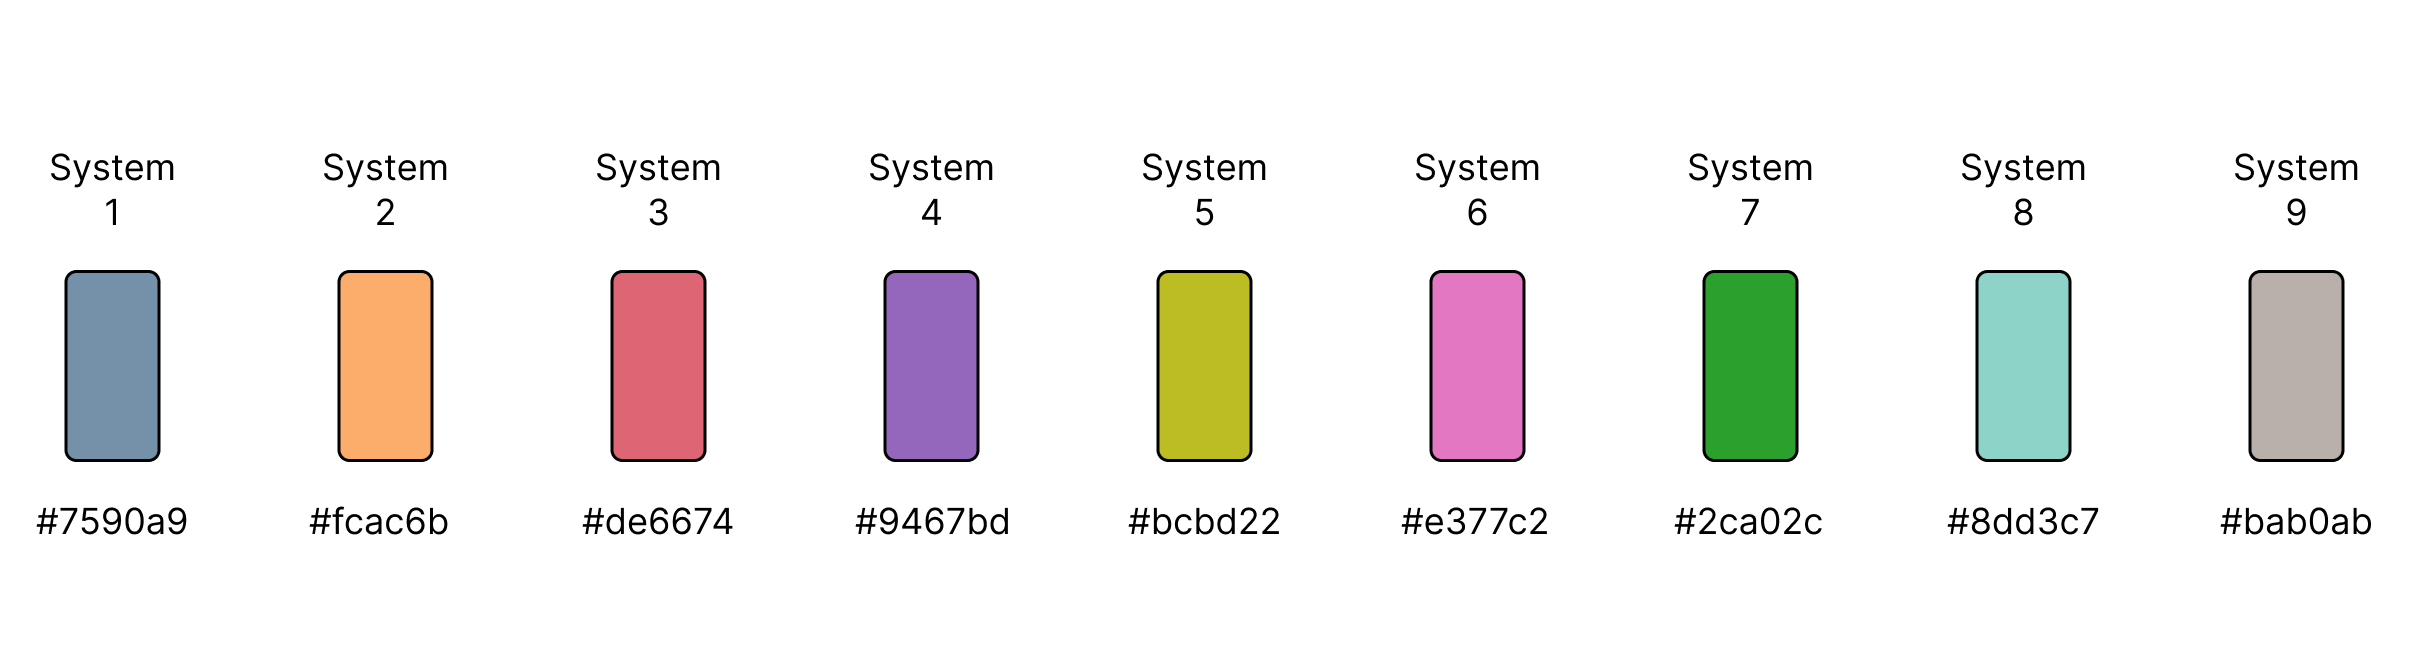
\includegraphics[width=1\linewidth]{figures/colors-dbms.png}
  \caption{Color palette used by visualizations.}
  \label{fig:colors-dbms}
\end{figure}

To enhance user experience, the Benchy Viewer incorporates immediate feedback mechanisms. When users hover over interactive elements, such as buttons or inputs, accent colors dynamically adjust, providing a visual cue of the interactive nature of the element. Additionally, the mouse representation undergoes subtle changes, reinforcing the responsiveness of the interface.\\
Additionally, the Benchy Viewer employs the Roboto font \parencite{roboto} for a clean and modern look, enhancing readability and contributing to a user-friendly interface.


\subsection{Page Structure and Navigation}\label{sec:page-structure}

The design of the Benchy Viewer is thoughtfully crafted for user convenience and simplicity. This section provides insights into the structural components that define the organization of the Benchy Viewer.

At the heart of the application's architecture are the header and the sidebar, ensuring constant visibility for users and facilitating seamless navigation. These elements contribute to maintaining a strong sense of orientation throughout the user journey.


\subsubsection{Sidebar}

The Benchy Viewer adopts a standard web view with a sidebar, leveraging the familiar layout seen in many web applications, as illustrated in Figure~\ref{fig:app}. This approach comes with inherent advantages. Users accustomed to web interfaces will find this structure intuitive and easily navigable, contributing to a seamless user experience.

\begin{figure}[h]
  \centering
  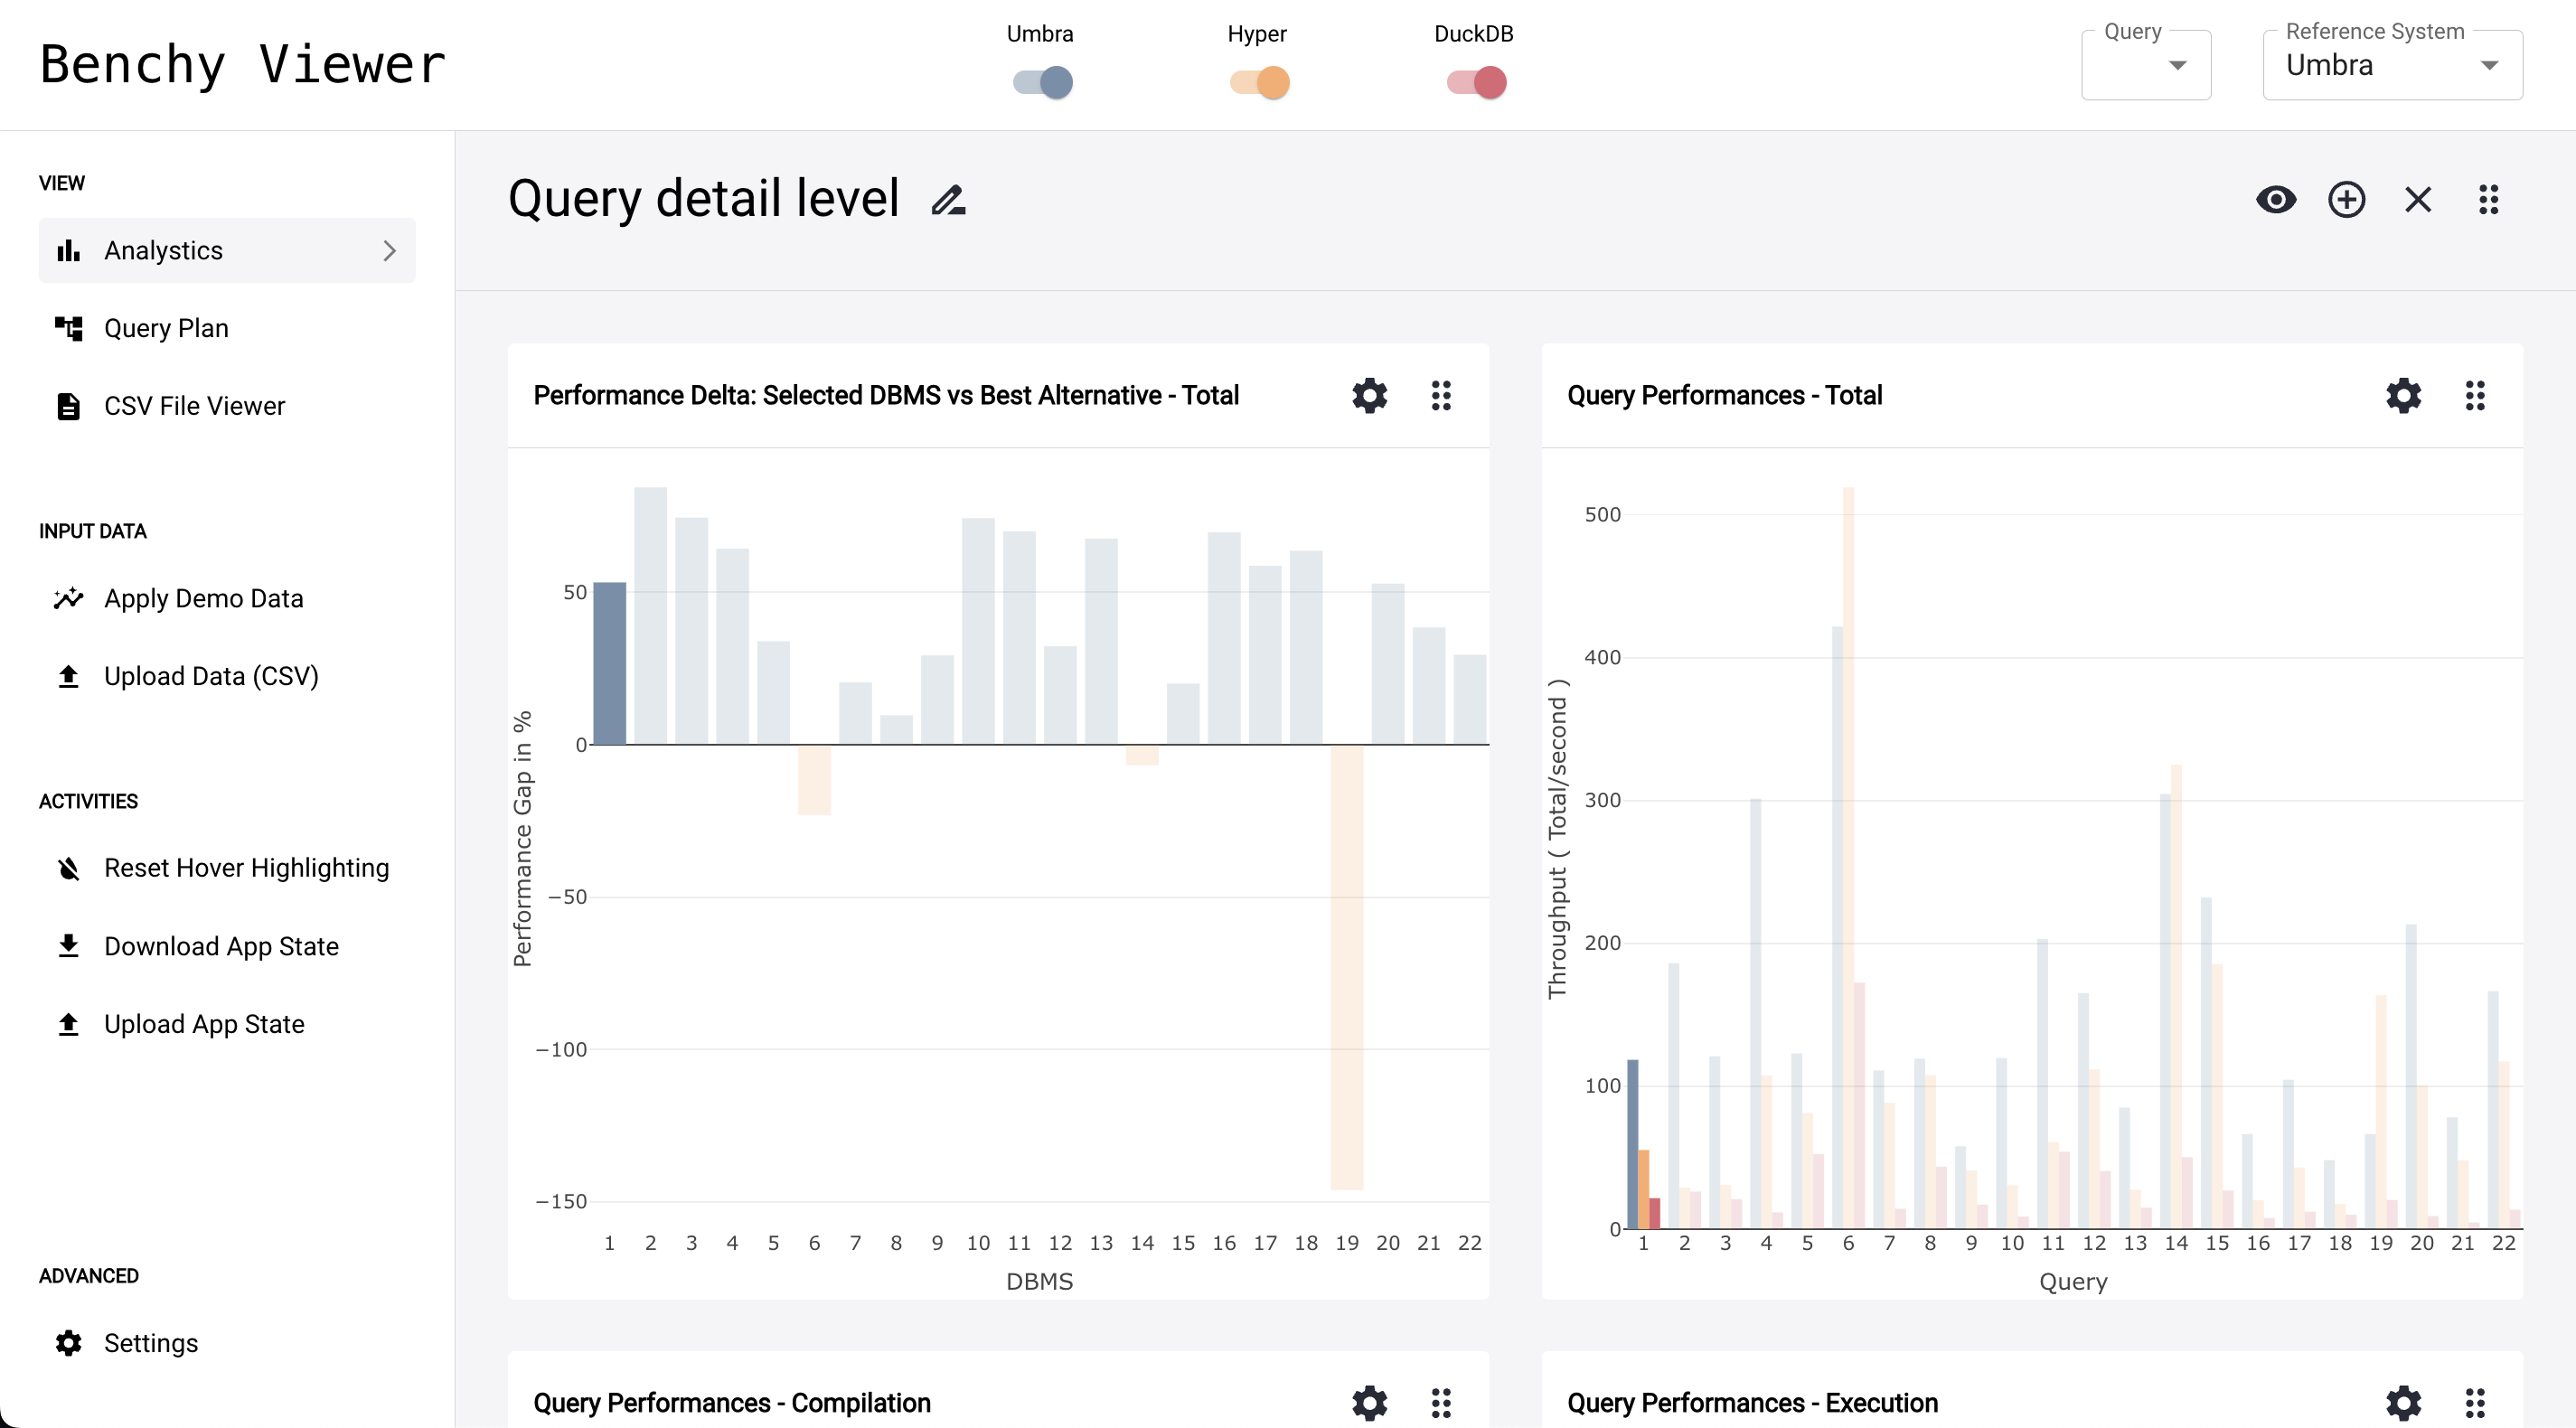
\includegraphics[width=1\linewidth]{figures/app.png}
  \caption{Overview of the application structure.}
  \label{fig:app}
\end{figure}

The sidebar serves as the central hub for navigating different sections of the application, while always staying present. By providing a navigation button section, users can effortlessly transition between pages, ensuring quick access to specific functionalities and data views. Additionally, the navigation button of the current page is highlighted with the accent color.

Below, the users have the possibility to import benchmark data or explore the application's capabilities using demo data. This feature facilitates a hands-on experience without the immediate need to provide personal datasets, making it convenient for users to evaluate the application's functionalities.

The sidebar offers additional functionalities, including the ability to reset hover highlighting. Users can download and upload the application state, enabling them to save configurations and share them or reload them for future sessions, which is further examined in \ref{sec:saving-sharing-state}. 

A settings icon button in the sidebar provides direct access to the global settings of the Benchy Viewer, allowing users to adjust application-wide settings from anywhere within the application.



\subsubsection{Header}
The header, along with the sidebar, remains visible in all scenarios within the Benchy Viewer. While the sidebar offers a range of functionalities, the header contains fewer elements. The central element of the header is the legend, strategically placed to eliminate the need for a legend in each individual visualization, promoting a clean and efficient overview. Users can activate or deactivate any system at any time using the toggles within the legend.

Another crucial functionality in the header is the selection of the baseline system and the focused query, offering the same advantage of accessibility at any point in the user's workflow.

Additionally, the header adapts contextually when navigating to the "Query Plan" page. In this scenario, a slider appears for selecting the comparison strategy between query plans, providing further flexibility and control, as explored in Section \ref{sec:semantic-diff-integration}.



\subsubsection{Pages}

The Sidebar and Header form the foundation of the user interface, while the remaining space is dedicated to displaying the various pages. Essentially, the Benchy Viewer comprises three main pages, depicted in Figure~\ref{fig:pages}: the Analytics Dashboard page, the Query Plan page, and the Input File Viewer page.

\begin{figure}[h]
  \centering
  \begin{subfigure}[b]{0.3\linewidth}
    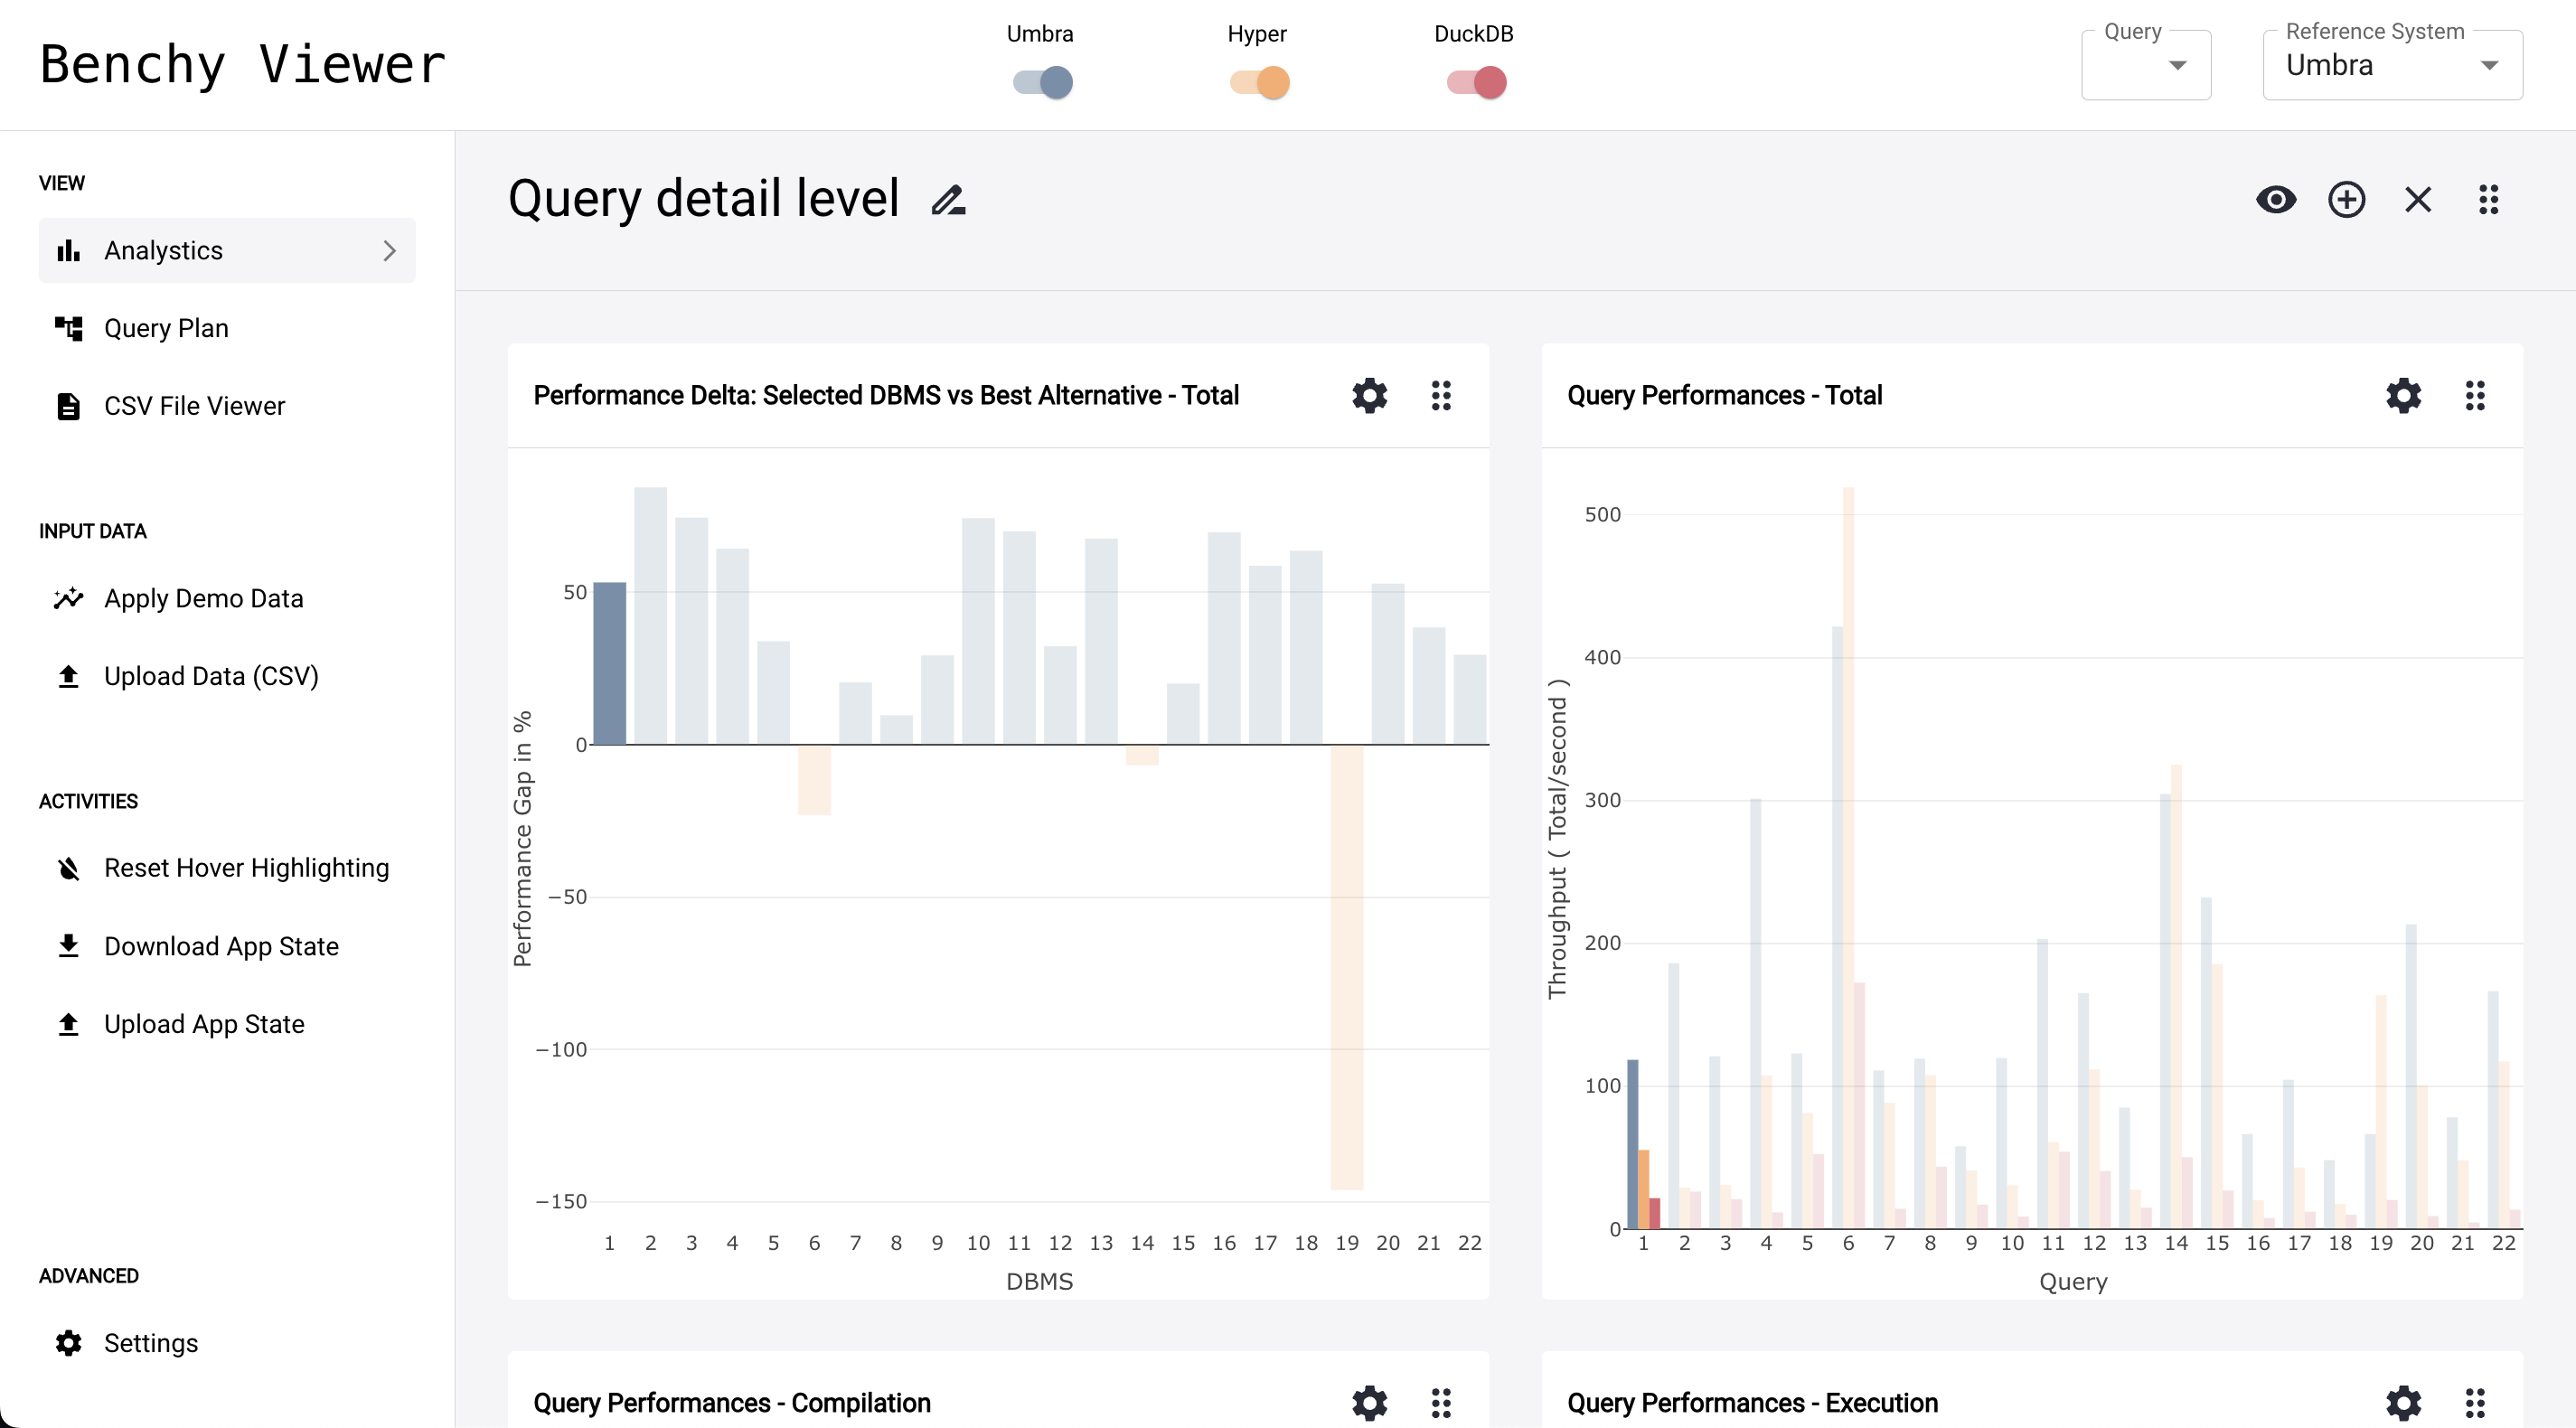
\includegraphics[width=\linewidth]{figures/app.png}
    \caption{Analytics Dashboard.}
      \label{fig:app-page}
  \end{subfigure}
  \hspace{0.5cm} % Adjust the horizontal space between the figures
  \begin{subfigure}[b]{0.3\linewidth}
    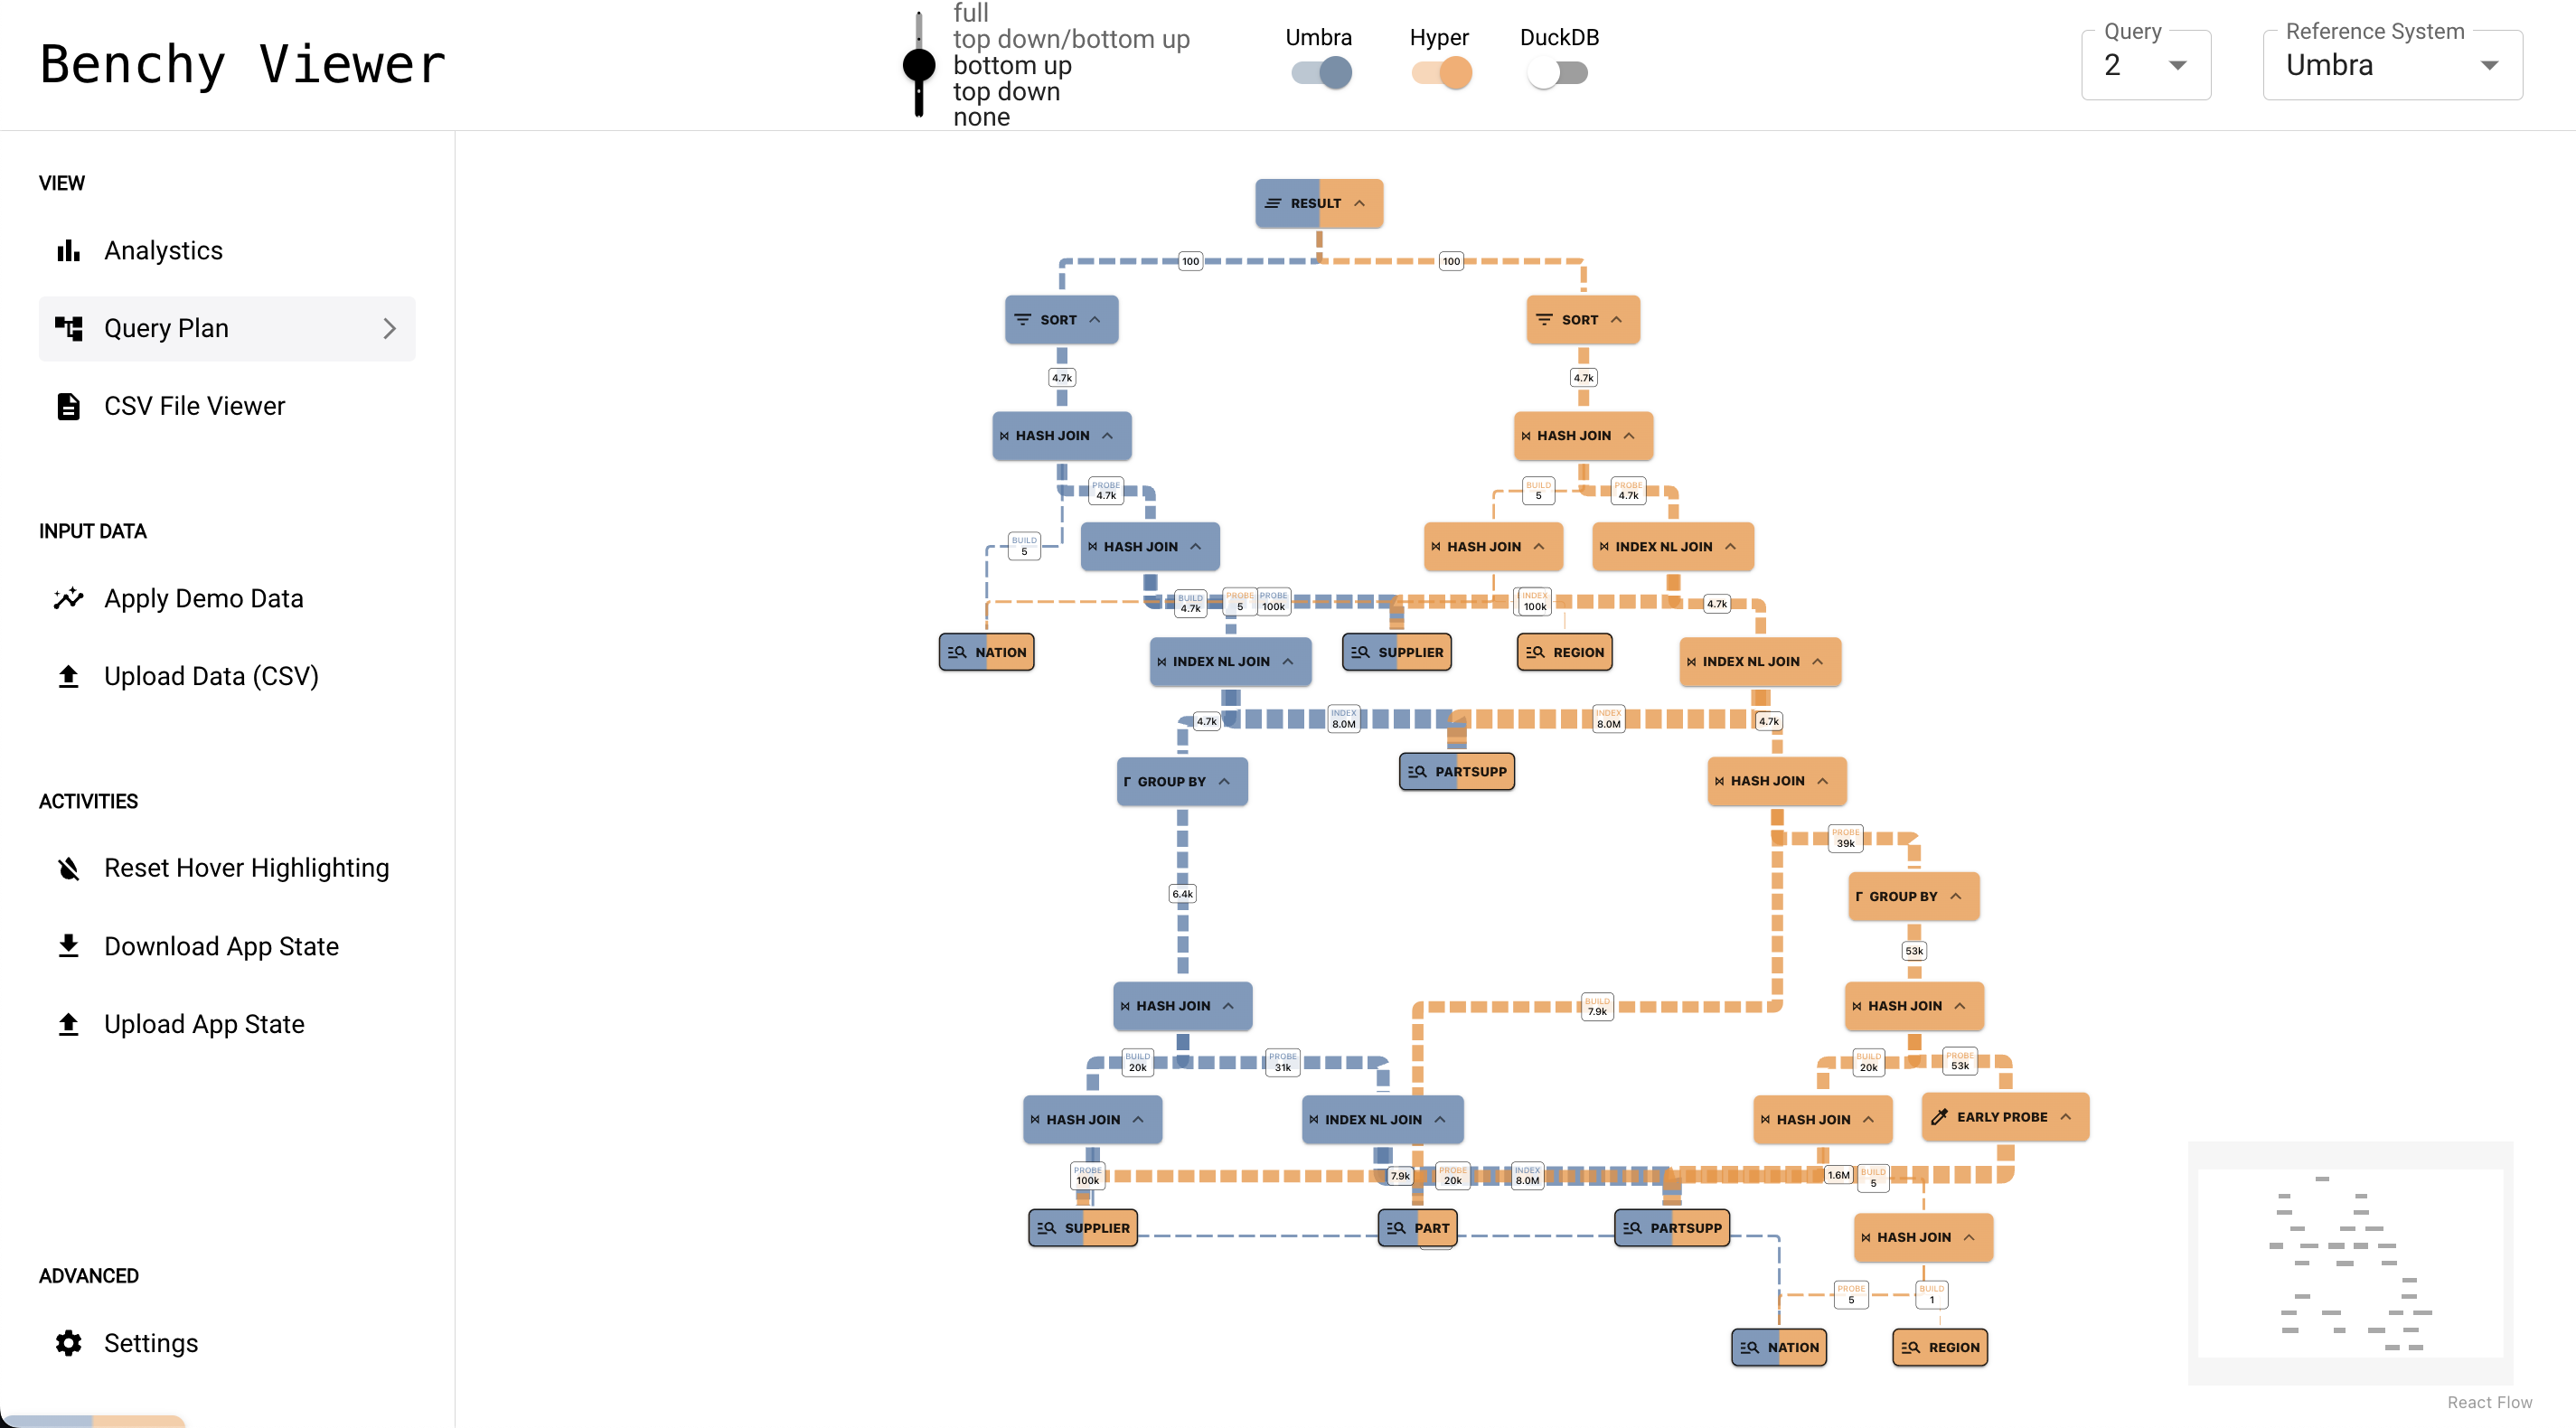
\includegraphics[width=\linewidth]{figures/app-query-plan.png}
    \caption{Query Plan View.}
      \label{fig:app-query-plan}
  \end{subfigure}
  \hspace{0.5cm} % Adjust the horizontal space between the figures
  \begin{subfigure}[b]{0.3\linewidth}
    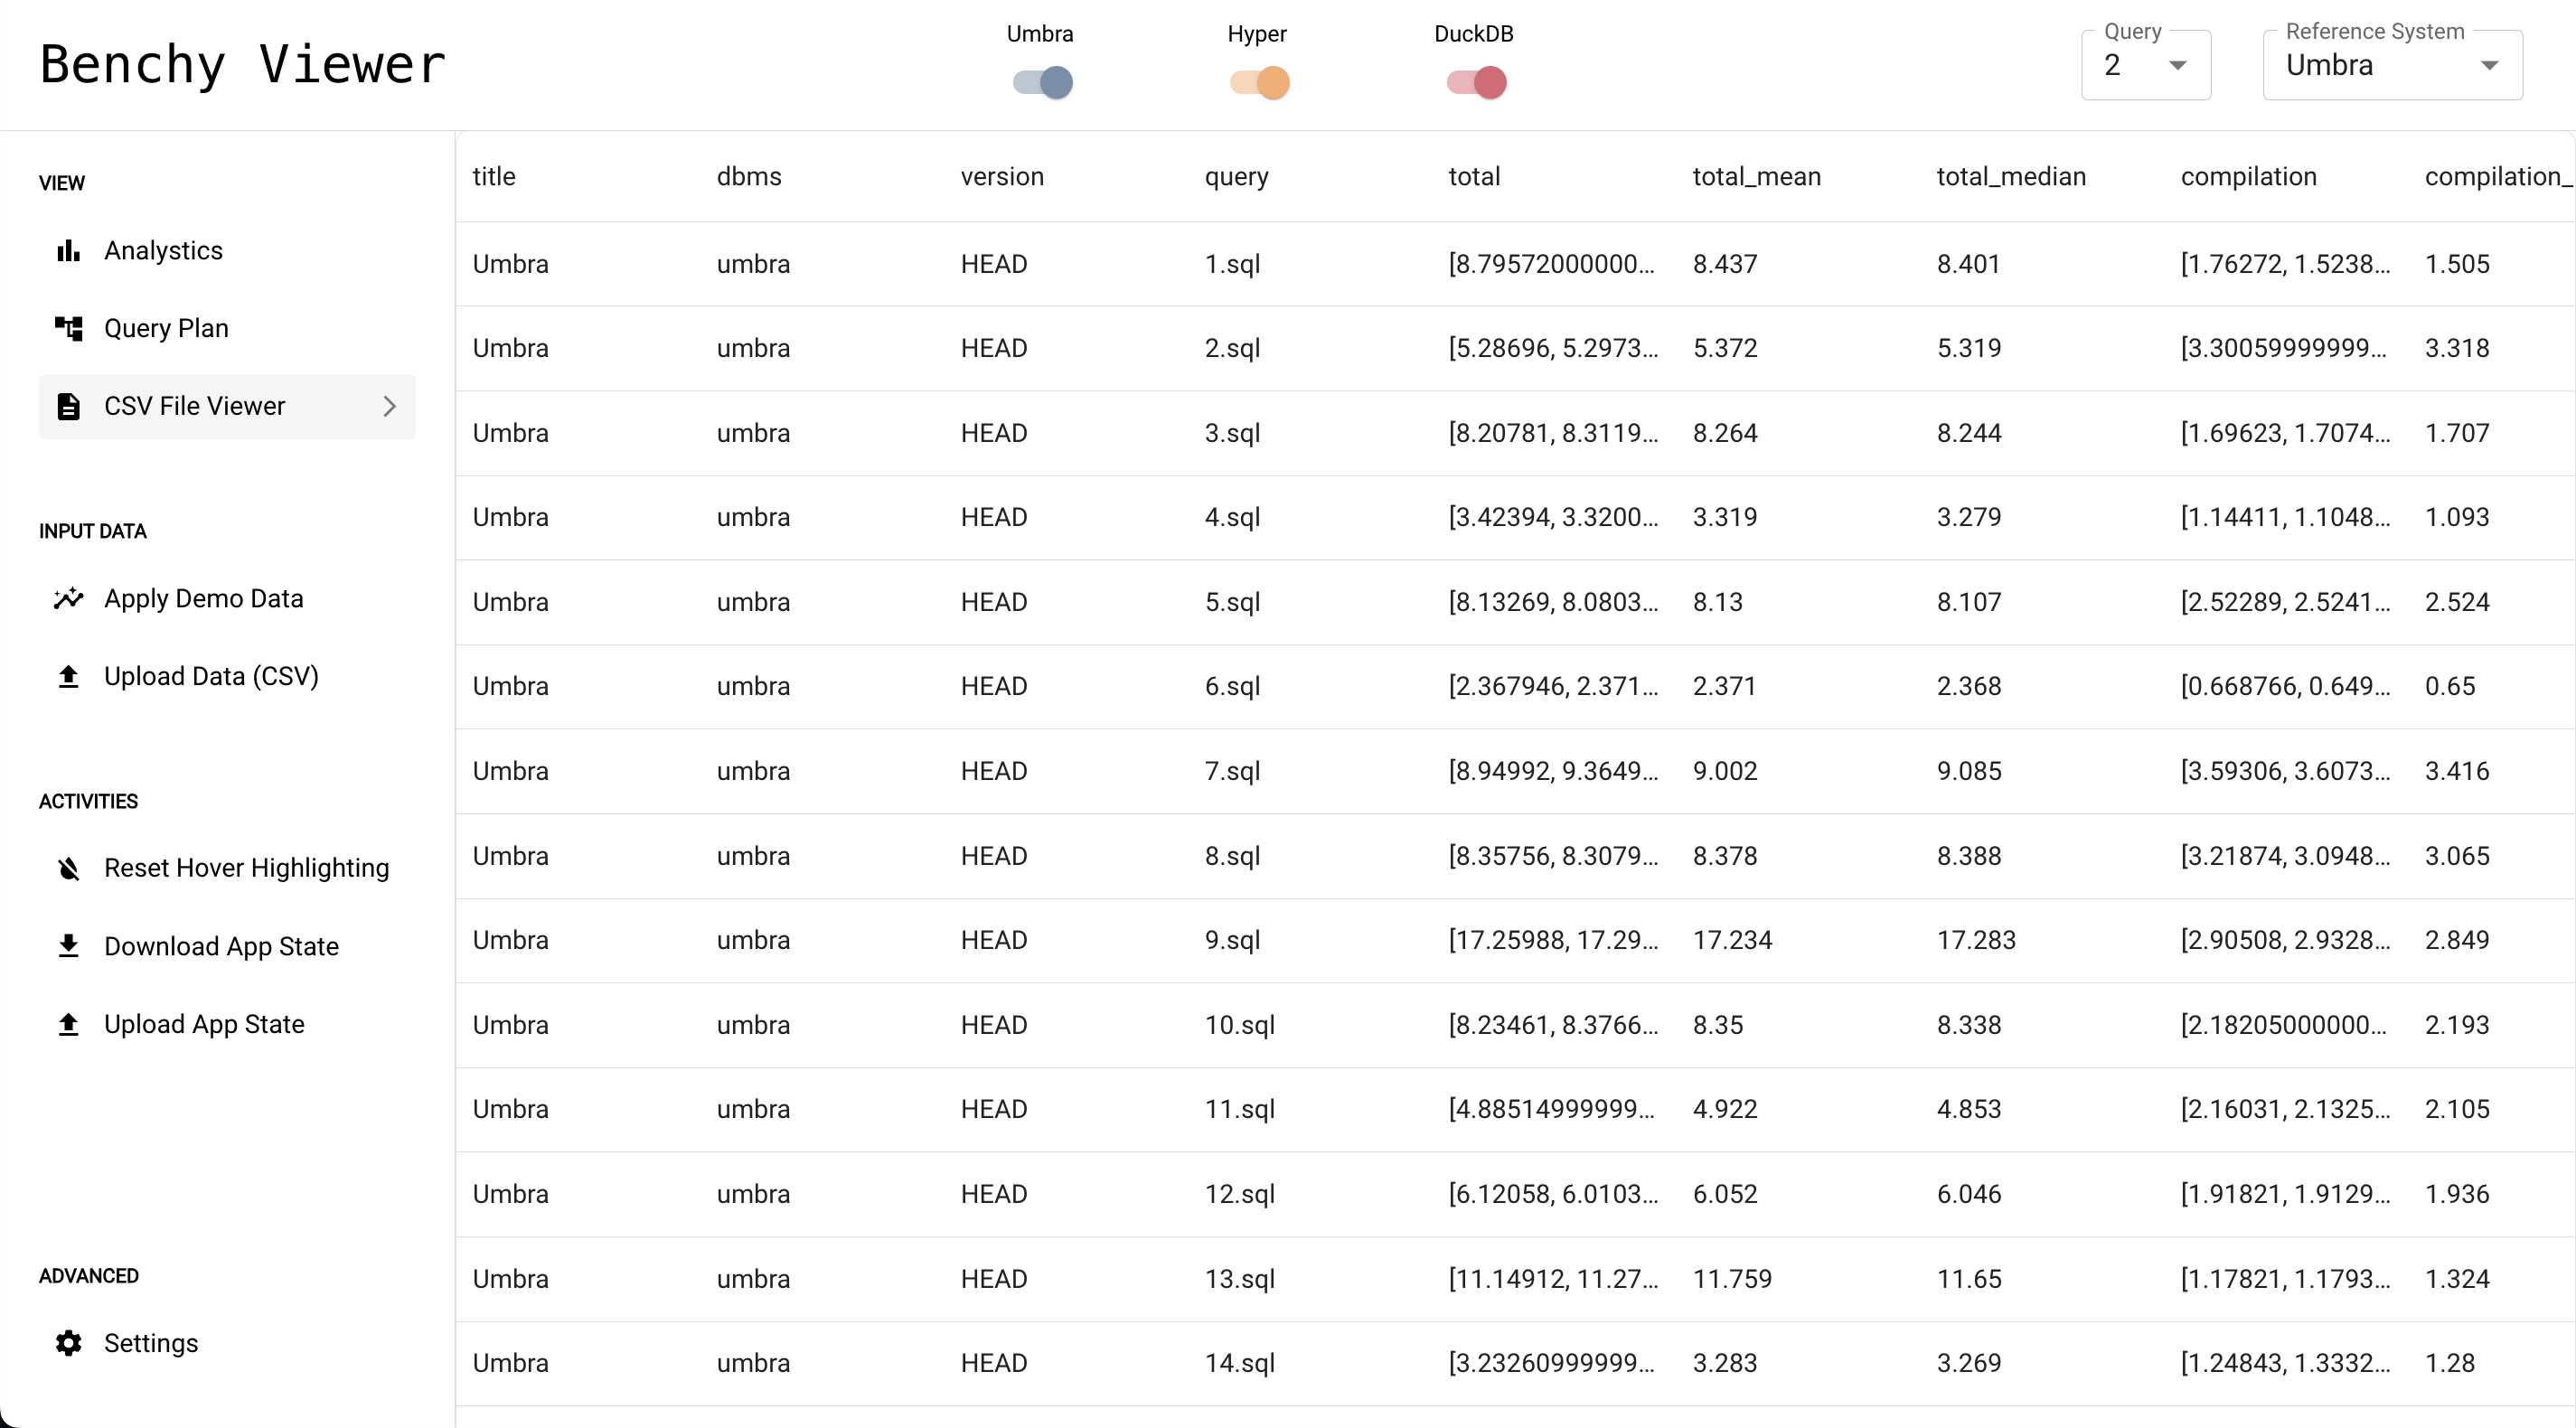
\includegraphics[width=\linewidth]{figures/app-data-viewer.png}
    \caption{Input File Viewer.}
      \label{fig:app-data-viewer}
  \end{subfigure}
  \caption{From left to right: Analytics Dashboard page, Query Plan View page, and Input File Viewer page.}
  \label{fig:pages}
\end{figure}

The Analytics Dashboard page features the drag-and-drop system for visualizing elements and their containers. This page serves as the hub for analysing benchmark data, offering charts and plots to explore queries from diverse perspectives.

Upon identifying significant queries using the analytics dashboard, users often transition to the Query Plan page. This page serves as a central hub for comparing distinct query plans across various database systems. 

In contrast, the Input File Viewer page offers a minimalist perspective. Tailored for users seeking an unembellished view of their imported benchmark data, this page omits visualizations. It provides an in-depth examination of the raw data, enabling users to scrutinize the dataset's structure and intricacies without the influence of charts or plots.















\section{Data Structure}
Unraveling the complexities of the Benchy Viewer necessitates a deep dive into its fundamental data structure, a cornerstone shaping the app's functionality and user interaction.\\
Our exploration commences with an examination of the broad project data structure, leading to a comprehensive exploration of each intricate facet of the global application state.

\subsection{Overall Project Structure}

The Benchy Viewer embodies a robust project structure that leverages React, global state management, and a page navigating router, as illustrated in Figure \ref{fig:project-structure}, which we will explore in this section.

\begin{figure}[h]
  \vspace{0.5cm}
  \centering
  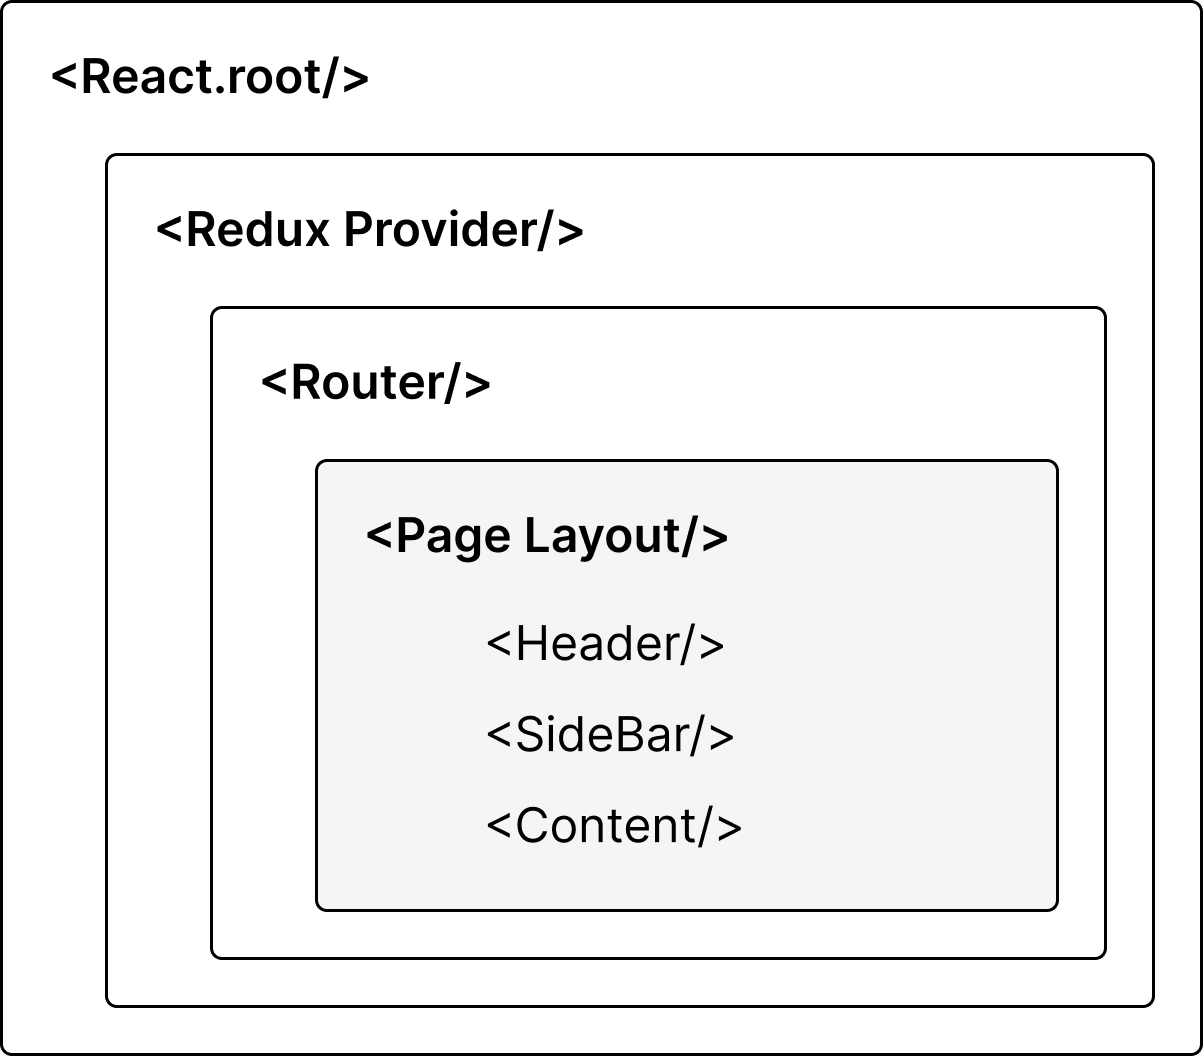
\includegraphics[width=0.5\linewidth]{figures/project-structure.png}
  \caption{Project Structure Hierarchy.}
  \label{fig:project-structure}
\end{figure}

\subsubsection{Root Component}
The root component is the entry point of the Benchy Viewer React application, orchestrating critical processes that define its robustness and efficiency.\\
The primary responsibility of the root component is to render the main application, serving as the nexus for various functionalities, providing the structural and organizational backbone for the entire application. 

In the project structure hierarchy, the root component encapsulates the application with\texttt{ <React.StrictMode/>}~\parencite{reactstrictmode}, which is a tool that highlights common issues and potential problems in a React application during development.
In general, it detects impure calculations in the context of component states and multiple rendering. It enables a set of additional checks and warnings to catch and alert developers about unsafe or deprecated practices, contributing to better code quality. While it doesn't affect the production build, it's a valuable aid in identifying and addressing issues early in the development phase.


\subsubsection{State Management with Redux}
The Redux Provider in the Benchy Viewer, built using Redux~\parencite{Redux}, serves as the central hub for managing the application's state. It acts as a shared space where different parts of the application can store and retrieve data efficiently.\\
Utilizing the capabilities of \textit{Redux Toolkit}~\parencite{redux-toolkit}, the Redux Provider supplies the global state across the entire application. This global state is compartmentalized into five distinct slices, illustrated in Figure~\ref{fig:global-state}, each serving a unique purpose.

\begin{figure}[h]
  \centering
  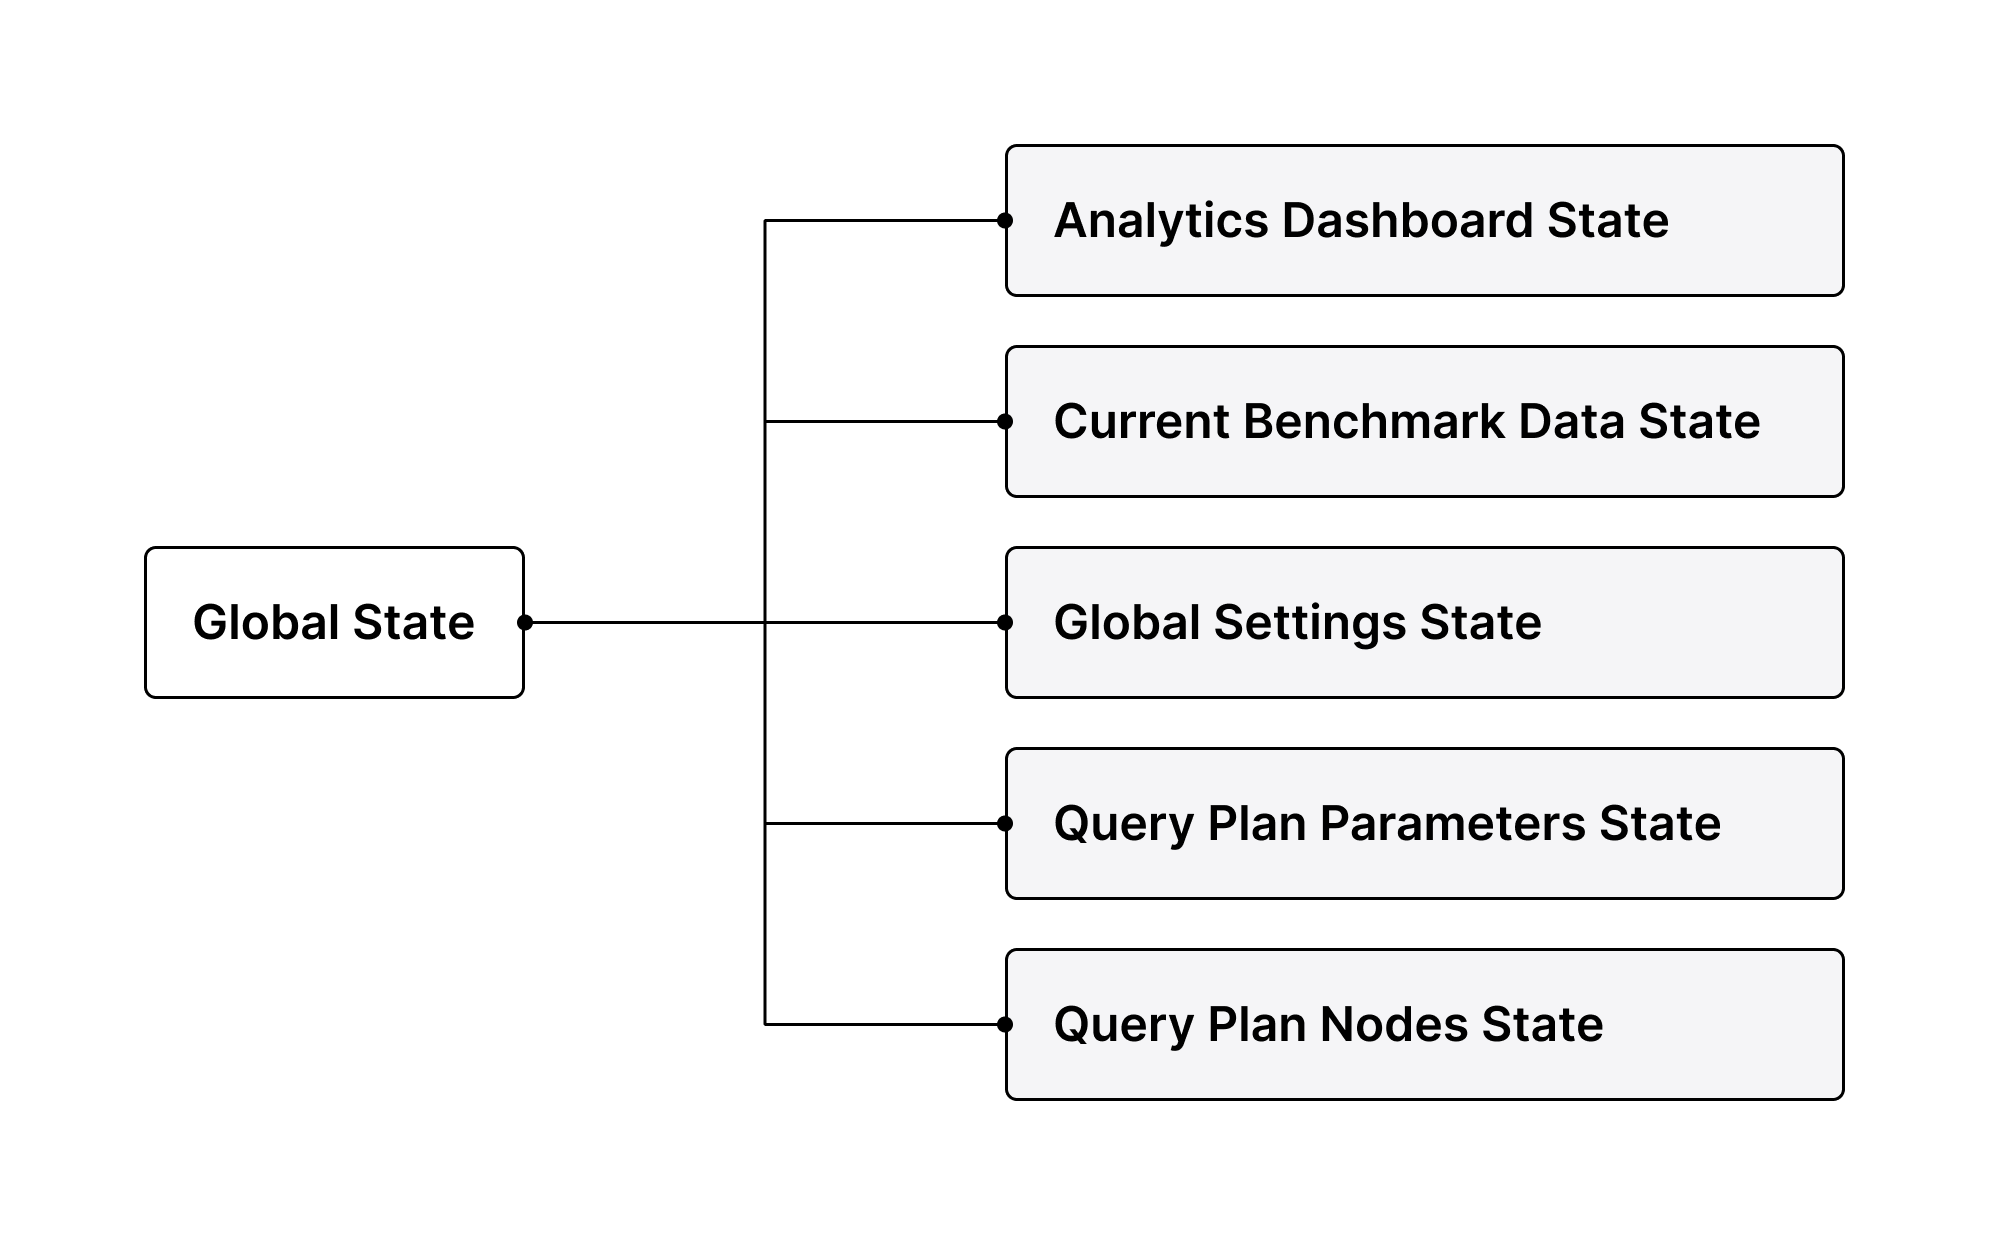
\includegraphics[width=0.8\linewidth]{figures/global-state.png}
  \caption{Application State Compartements.}
  \label{fig:global-state}
\end{figure}

% Analytics Dashboard state
The Analytics Dashboard State encapsulates all the data concerning visualizations within the Analytics Dashboard. It includes information about the position within the dashboard and the configuration of each visualization element. A more detailed exploration of this data structure is provided in Section \ref{sec:analytics-dashboard}.

% Imported Benchmark Data state
The Current Benchmark Data State is responsible for holding all benchmark data from various database systems. This state is a pivotal component used across the Analytics Dashboard, Query Plan View, and Benchmark Data View. A detailed examination of this state's structure is available in Section \ref{sec:input-data}.

% Global Settings state
Focused on interactive features within visualizations, the Global Settings State encompasses functionalities like the global hover state or the selected query. Section \ref{sec:global-settings} delves into the specifics of this data structure.

% Query Plan Parameters state
Tailoring the visualization needs for the user, the Query Plan Parameters State contains data related to the appearance and comparison types of the query plans. More insights into this state are provided in Section \ref{sec:query-plan-parameters}.

% Query Plan Nodes state
Lastly, the Query Plan Nodes State unfolds the story of the actual query plan, housing details about every node and their associated information. For a comprehensive exploration, turn to Section \ref{sec:query-plan-structure}.


\subsubsection{Router}
Navigating through the corridors of the Benchy Viewer's project structure, the router, powered by \textit{React Router} \parencite{react-router}, providing a standardized approach to handle navigation in React. Specifically, in our application, this router guides users through three key areas: the Analytics Dashboard, Query Plan View, and Data Viewer.

\subsubsection{Layout and Content}
Finally, we encounter the pages with their contents within the Benchy Viewer. These pages share a consistent structure, ensuring a unified user experience. Each page adheres to a standardized layout, featuring a sidebar, a header, and a dedicated space for content, which we discussed the page structure in \ref{sec:page-structure}.

At this point, the various components at different levels come together to form the Benchy Viewer application. The root component lays the groundwork, overseeing essential processes. The Redux Provider acts as a central hub for sharing information across the application. The global state, divided into five slices, provides state to all pages. The router facilitates easy navigation between pages, which is controlled in the sidebar. In essence, these pages, with their structured layouts, unite to offer users a seamless and comprehensive experience.














\subsection{Benchmark Data}\label{sec:input-data}

The initial step when engaging with the Benchy Viewer involves importing a file containing performance data slated for visualization. This file must adhere to the format outlined in Section \ref{sec:input-file-structure} and is processed by the Current Benchmark Data State, introduced in the previous section. 

\subsubsection{Import Process}

Throughout the importation process, the input file undergoes parsing and transformation into a TypeScript object. Subsequently, the benchmark data is partitioned according to the respective database systems. This partitioning ensures that all query data aligns with its associated database system. The resulting data structure encompasses a system ID, a title, all pertinent benchmark data, and an activation flag.

\subsubsection{Data Accessibility}

After the data import, the benchmark data is accessible to all visualization elements across the whole application. This includes all visualization elements within the Analytics Dashboard, the Input File Viewer, and the Query Plan View.

The activation flag controls the visibility of the system data of a whole database system in the visualizations. This is accessed through the header's legend toggles, where users can control the activation or deactivation of database systems.

Additionally, this state holds the demo data, which is initialised on the start of the application. Upon user requests via the sidebar, the demo data is loaded as the current benchmark data.



\subsection{Global Settings}\label{sec:global-settings}

In the Benchy Viewer, the global settings serve as a central hub for interactive and customizable data exploration. Features like hover and selected queries offer real-time insights, while selecting a baseline system deepens understanding for comparative analysis. Visual configurations provide the power to mould data representation, aligning with user preferences. In essence, the global settings act as the control center, empowering users for dynamic and tailored data exploration.

\subsubsection{Hovered Query}

A key interactive feature is the global hover functionality, where details about the currently hovered query are stored. This information is triggered when a user hovers over a specific query within a visualization element on a detailed level, like a bar in a bar chart. This hover information is then synchronized across all other visualizations simultaneously.

\subsubsection{Selected Query}

Much like the hover feature, the selected query is stored and activated through interactions within the visualization elements at a detailed level. Additionally, a drop-down input in the header allows users to manually select the current query. This state is utilized not only for highlighting purposes in the Analytics Dashboard, but also in the Query Plan View for selecting the corresponding query plan.

\subsubsection{Baseline System}

Another crucial component within this data slice is the selected baseline system, a linchpin for comparative analyses in the Benchy Viewer. This feature empowers users to delve into the results of their chosen system, comparing and contrasting its performance against other systems. This is particularly valuable in visualizations incorporating metrics like speed-up and slow-down.

Specifically utilized in visualizations such as the comparative query bar chart, the selected baseline system plays a vital role in illustrating the performance delta for each query. This allows users to discern the nuanced differences between the baseline system and the best-performing alternative. 

\subsubsection{Visualization Configurations}

This segment houses configuration options influencing the visual aspects of charts, detailed in Section \ref{sec:chart-configuration}. It governs factors like the chart axis scale and display type for violin plots. Users can conveniently access and tweak these options through the settings menu in the sidebar. The choices made here resonate across various visualization elements in the Analytics Dashboard, providing a tailored and cohesive visual experience.










\subsection{Analytics Dashboard Data Structure}\label{sec:analytics-dashboard}

The Analytics Dashboard in the Benchy Viewer acts as a central hub for comprehensive performance analysis, providing a structured and user-friendly interface. At its core, the data structure slice forms the backbone, storing essential information about analytics sections and the visual elements they contain.

\subsubsection{Containers}
This data slice manages a roster of analytics sections, with their order mirroring the sequence in the UI's drag-and-drop system. Reordering the analytics sections in the UI through the drag-and-drop feature will update this state.

Each container in the list retains a name for labeling the analytics section. Additionally, a visibility flag dictates whether the container is collapsed or its content, along with all its charts, is visible. In general, all of these properties are accessible in the UI through the containers header.\\
Lastly, every container holds a list of its associated visualization elements. 

\subsubsection{Visualization Element}
Within each container, a list of visualization elements is stored, aligning with the sequence in the UI's drag-and-drop system. Reordering charts in the UI through the drag-and-drop feature will update this state.

These visualization elements are distinguished by a label in their header, signifying their content.\\
Furthermore, each element is characterized by a property denoting its visual type, such as a bar chart or violin plot.\\
Lastly, a vital attribute is the metric associated with each visualization element, such as execution time or compilation time. In the UI, this is accessible through the chart menu, see \ref{sec:chart-configuration}.





\subsection{Query Plan}
The incorporation of the query plan into the Benchy Viewer relies heavily on the integration of the Query Plan Visualizer \parencite{semantic-diff}. For a more detailed exploration of this integration, refer to Section \ref{sec:semantic-diff-integration}.

The query plan's data structure is divided into two essential parts. First, there are parameters governing the visual aspects and comparison strategies of the query plans. Second, we have the actual query plan data for the database systems.

\subsubsection{Visualization Parameters}\label{sec:query-plan-parameters}

To enhance the user experience, the Query Plan Viewer incorporates a collapsible functionality in every node, denoted by an icon. The activation of this functionality at a specific node will collabse its whole subtree.\\
Recognizing that some users may find this feature unnecessary, an option exists in the settings to disable collapsibility. This choice hides all icons in the nodes, ensuring a cleaner and less distracting look for the query plan.

The matching algorithm parameter is a pivotal component influencing the visualization of query plans in the Benchy Viewer. This property, structured as an enum, provides a spectrum of options to tailor the matching algorithm based on specific visualization needs. It is accessible in the header when the Query Plan View is active, as depicted in Figure~\ref{fig:query-plan-slider}. When set to "none", it allows query plans to be displayed independently, side by side, without any comparison. Alternatively, choosing "top down" or "bottom up" initiates matching algorithms that prioritize either a top-down or bottom-up approach, optimizing clarity in specific scenarios. The "top down/bottom up" option combines both methods, offering a balanced approach.

Lastly, users have the option to customize the visualization of edges within the query plan. By default, edges are presented in horizontal and vertical directions, reminiscent of a classical tournament tree. However, when dealing with intricate query plans or non-planar graphs, overlapping edges may compromise clarity. To address this, users can modify the edge style. This customization allows edges to deviate from strict horizontal or vertical orientations, adopting a more dynamic style that allocates additional space to each edge. This flexibility ensures that the visual representation of edges aligns with the structure of the query plans, contributing to a more informative visualization.



\subsubsection{Query Plan Data Structure}\label{sec:query-plan-structure}

During the import of benchmark data into the Benchy Viewer, the query plan metadata undergoes a transformation process to populate a structured object. This involves parsing the raw metadata provided in the benchmark results, which includes details such as the operator ID, estimated cardinality, and exact cardinality.

The data transformation involves creating instances that represent each element of the query plan, forming a tree structure to reflect the hierarchical arrangement. This establishes relationships between elements to capture the flow and nesting of operations. System-specific details are retained within each node throughout this transformation. This structured representation enables users to navigate the intricacies of the query execution flow.








\section{Integration of Plotly-React for Data Visualization}
For visualizing the data within plots and charts, the graphing library \textit{Plotly} \parencite{plotly}, was used. Plotly is a versatile and interactive graphing library widely used for data visualization. Its compatibility with languages like JavaScript, through \textit{Plotly JavaScript} \parencite{plotly-js}, enhances its appeal for web-based applications. With its features and user-friendly interface, Plotly is a solid choice for rendering interactive visual representations of data.

\subsection{General Features}
Plotly comes out of the box with a bunch of features that align with the interactability of the Benchy Viewer.

Plotly allows users to effortlessly scroll, zoom, and pan around plots, offering a dynamic exploration of the data. The ability to reset zoom provides added convenience, ensuring users can navigate through intricate details with ease.\\
Plotly further extends its functionality by enabling users to download the current representation as a PNG file, facilitating seamless sharing and documentation of visual insights.\\
The interactive hover feature adds another layer of depth to the visualization, allowing users to access specific data points with a simple cursor hover. The hover feature in Plotly was used to form the global hover feature, which we will discuss further in \ref{sec:plotly-hover}.





\subsection{Integration of the Global Hover Feature}\label{sec:plotly-hover}

Plotly offers great customization capabilities to developers, particularly when interacting with data points through the hover feature. When hovering over data points, Plotly provides detailed information, including the value and index. This hover information undergoes filtering, where the resulting query number is sent to the corresponding data slice. 

\begin{figure}[h]
  \centering
  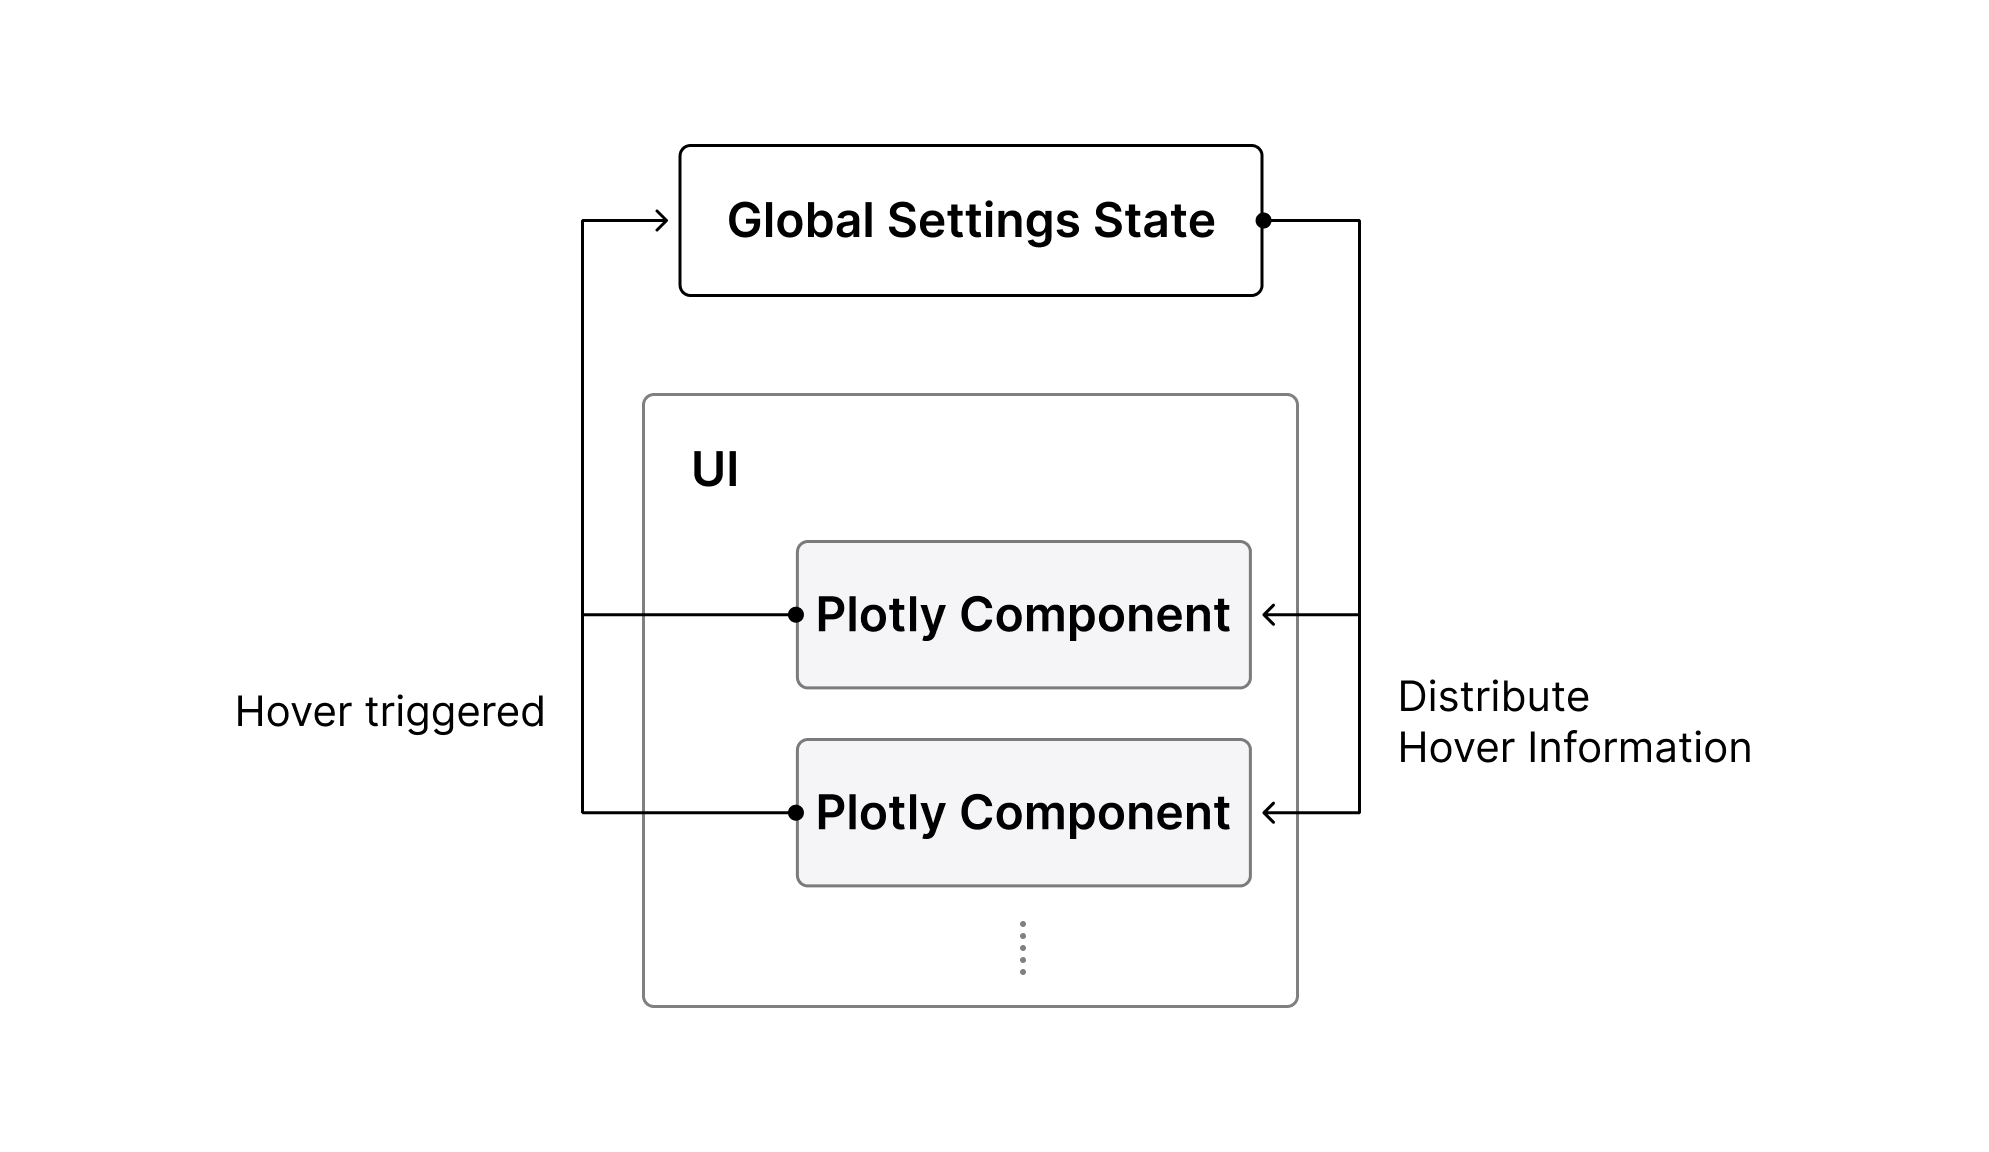
\includegraphics[width=0.8\linewidth]{figures/global-hover.png}
  \caption{Distribution of the Hover Information.}
  \label{fig:global-hover}
\end{figure}

Subsequently, the UI is automatically updated, and the hover information is distributed to all Plotly components. This dynamic process ensures that the queries associated with the provided information are highlighted, creating a synchronized and insightful data exploration experience. For a visual representation of this data flow, refer to Figure~\ref{fig:global-hover}.

\subsection{Wrapper Component providing necessary Properties}
To ensure seamless integration and synchronized functionality with the Benchy Viewer, Plotly components are encapsulated within a specialized wrapper component. This wrapper, illustrated in Figure~\ref{fig:chart-wrapper}, incorporates essential features.

\begin{figure}[h]
  \centering
  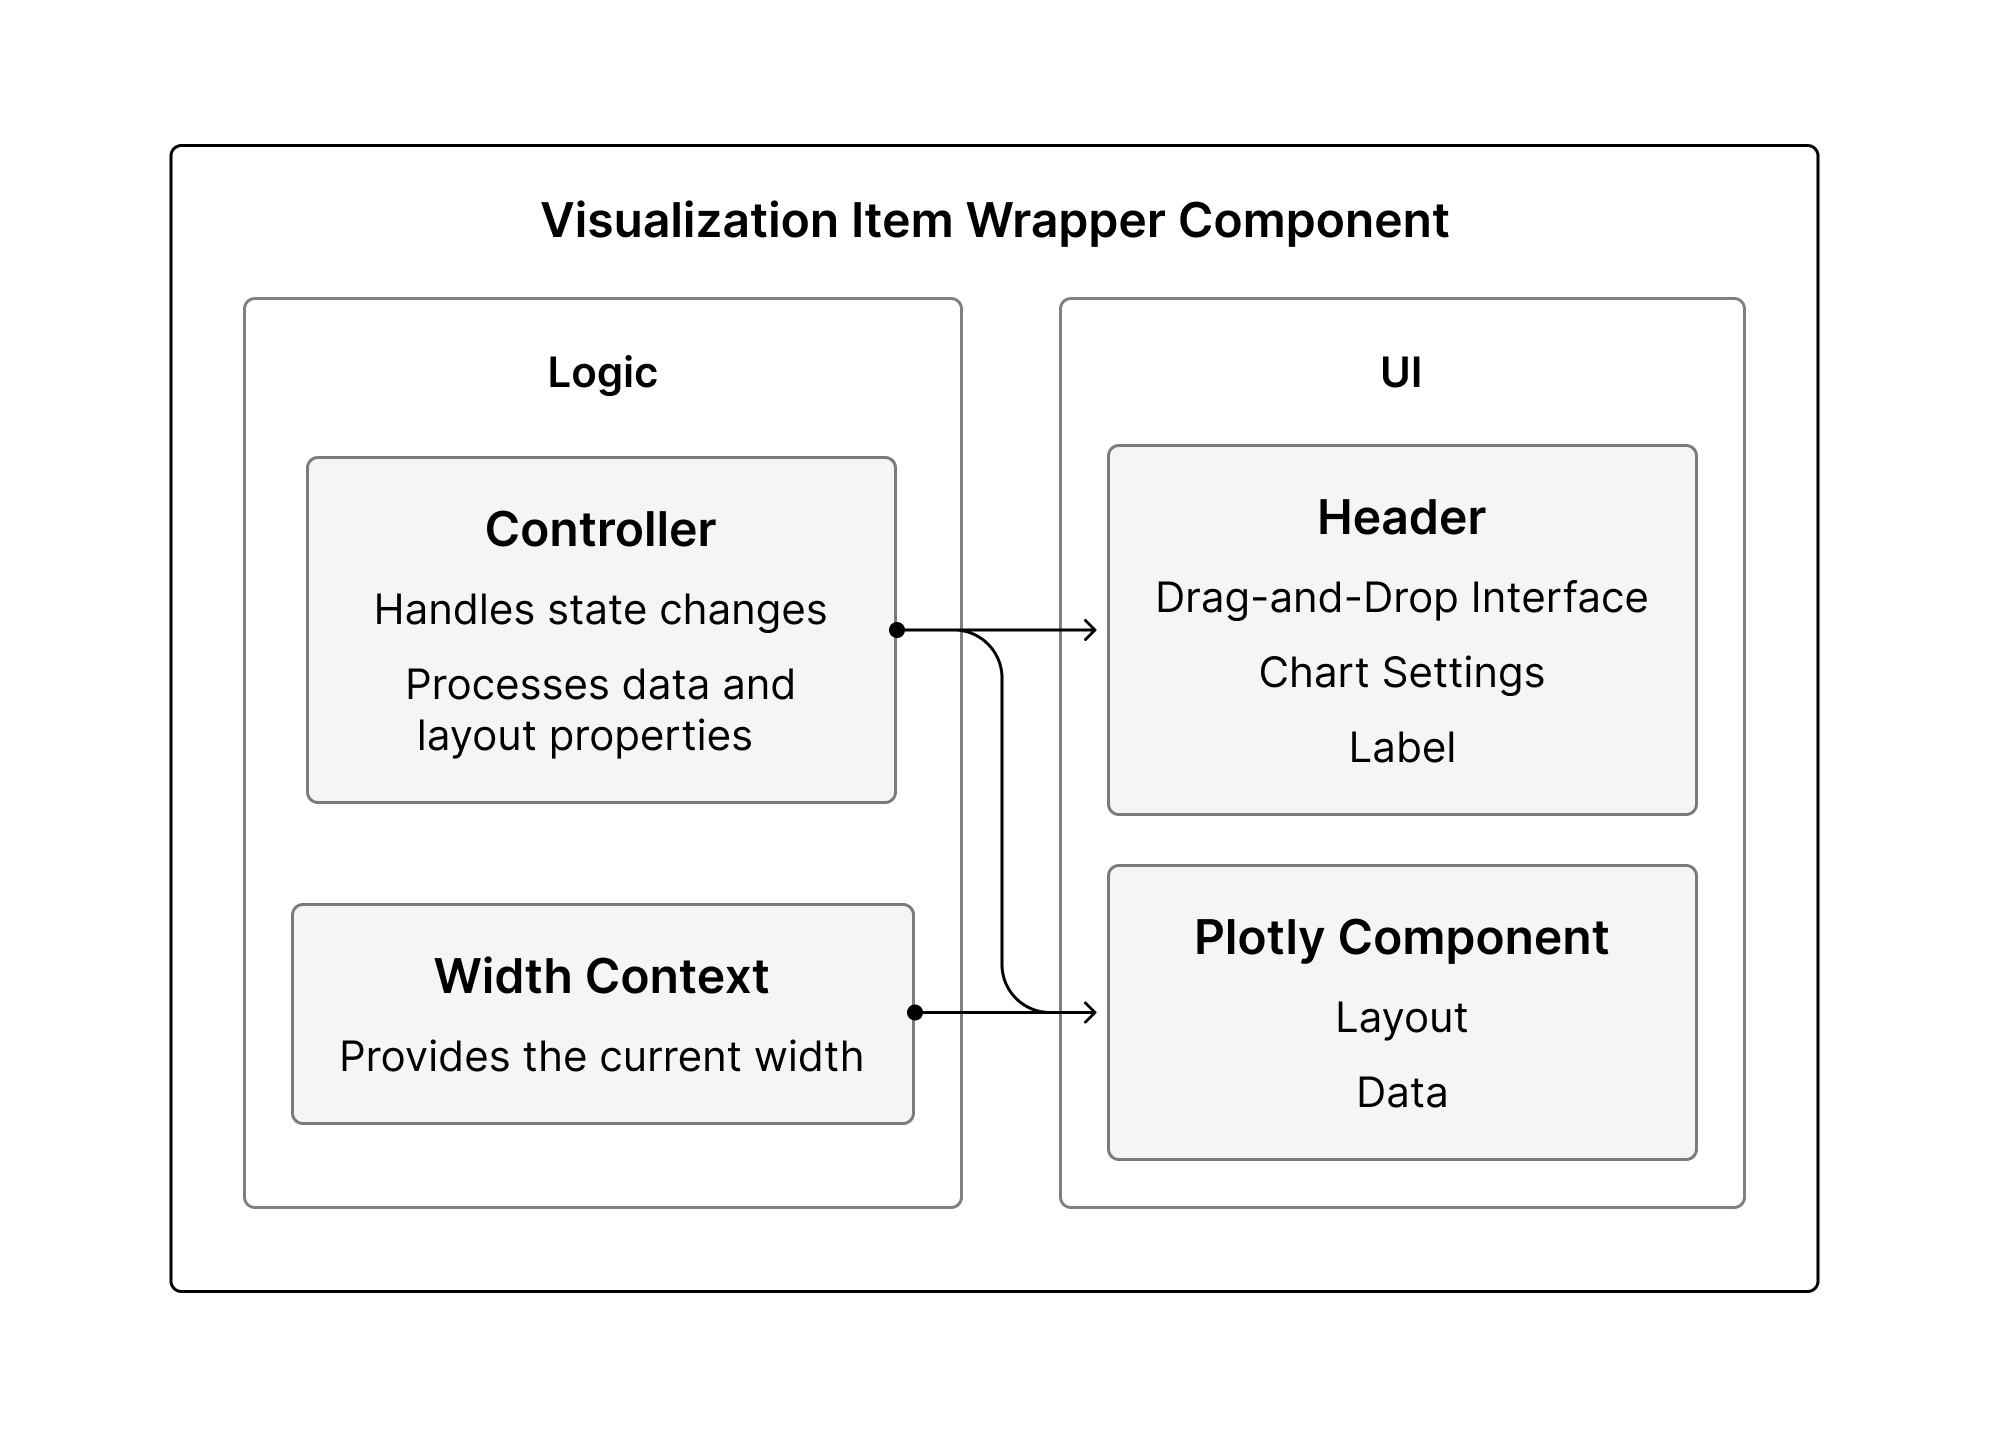
\includegraphics[width=0.6\linewidth]{figures/chart-wrapper.png}
  \caption{Wrapper Component Structure.}
  \label{fig:chart-wrapper}
\end{figure}

Firstly, it constructs the chart header, facilitating a drag-and-drop interface that seamlessly aligns with the Analytics Dashboard's drag-and-drop functionality. The header also encompasses chart settings, including a nested menu where users can select metrics and perform basic actions like duplication or deletion. Additionally, a descriptive label elucidates the content of the visualization element.

All the information presented in the wrapper is orchestrated by the controller, which manages state changes, such as when a user selects a different metric in the chart settings.\\
The controller is also responsible for preparing the data for visualization which involves the conversion of benchmark data into a data structure compatible with Plotly. This process may be divided into multiple stages, especially when utilizing metrics like speed-up and slow-down, which require additional calculations before presenting data to Plotly.\\
Calculations for proper scaling on the x-axis and y-axis are performed, taking into account the dataset's highest values. Furthermore, the controller constructs appropriate axis properties, such as the proper tick values, based on the visualization type and chart settings.

A notable consideration is that Plotly components expect concrete values for width and height. To accommodate varying screen sizes and dynamic resizing, the Benchy Viewer employs the React concept \textit{createContext} API \parencite{createContext} to form the \texttt{Width Context}. The implemented mechanism monitors the current width of the component and the \texttt{Width Context} propagates it down the component hierarchy. The mechanism, attuned to window resizing events, ensures that all components using the width prop from the \texttt{Width Context} are updated whenever the window size changes. This dynamic approach enables Plotly components to adapt effectively to different screen sizes and resizing scenarios.








\section{Integration of the Query Plan Visualizer}\label{sec:semantic-diff-integration}
Integrating the Query Plan Visualizer into the Benchy Viewer presented a challenge due to differing global state management systems. The Query Plan Visualizer uses React Sweet State \parencite*{react-sweet-state}, while the Benchy Viewer relies on Redux \parencite*{Redux}.\\
In the Business Logic subsection, we discuss the conversion process from React Sweet State to Redux. This involved a top-level restructuring to align with Redux's global state management, while maintaining application functionality.

In the UI subsection, both tools utilize the Material UI framework \parencite*{mui}, facilitating seamless code reuse. We highlight the reuse of Material UI components, like sliders, and the unique features of the Benchy Viewer's header, emphasizing code consistency with the reuse of components.


\subsection{Business Logic}

The integration of the Query Plan Visualizer into the Benchy Viewer introduced a challenge due to the disparity in the global state management systems used. The Query Plan Visualizer relies on React Sweet State for managing its state, encompassing everything from the actual query plan data to various configuration settings. On the other hand, the Benchy Viewer employs Redux for managing the global state of the entire application.\\
To maintain coherence and prevent the use of multiple state management tools within the application, a crucial step was to convert the relevant parts of the React Sweet State to Redux. This conversion process was a key challenge given that React Sweet State and Redux, while both state management libraries for React, have distinct approaches and underlying concepts.

The conversion process from React Sweet State to Redux involved a top-level restructuring of the state management logic. In React Sweet State, the state management is more localized and hook-based, catering to the component's specific needs. On the other hand, Redux operates with a global store and relies on actions and reducers for state modifications.

To migrate, we first identified the distinct states managed by React Sweet State and refactored them into Redux actions and reducers. This required careful consideration of how data flows through the application and the structure of the Redux store. The hook-based state management in React Sweet State was replaced with action dispatches and selectors in Redux.

Overall, the conversion aimed at preserving the application's functionality while aligning with the global state management paradigm of Redux. The resulting Redux implementation provides a successfully centralized state management system.


\subsection{UI}

The integration of both the Benchy Viewer and the Query Plan Visualizer with the Material UI framework facilitates a seamless UI integration process by allowing the reuse of substantial portions of the source code. Specifically, the Benchy Viewer has effectively repurposed various Material UI components, including sliders utilized for configuring the query plan and nodes in constructing the query plan.

Despite the Query Plan Visualizer boasting an extensive header with a multitude of functionalities, the Benchy Viewer adheres to a minimalist design, featuring only the most essential operations. To maintain this design philosophy, we identified the pivotal configuration features for the query plan within the Benchy Viewer's header. Any additional configurations were logically placed in the settings menu, accessible through the sidebar. In the Query Plan Visualizer, the activation and deactivation of query plans for database systems were accomplished using a Material UI Chip component \parencite{mui-chip}. While replicating this functionality was an option, we opted for reusing the header legend from the Analytics Dashboard, as depicted in Figure~\ref{fig:legend-conversion}. For this functionality, the legend provides its intuitive toggles with the corresponding system color.

\begin{figure}[h]
  \centering
  \vspace{0.5cm}
  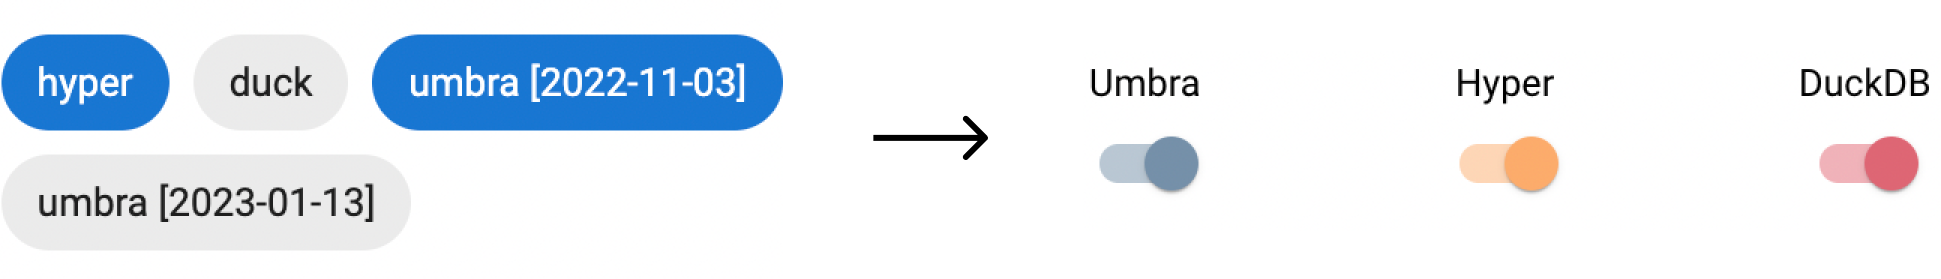
\includegraphics[width=0.8\linewidth]{figures/legend-conversion.png}
  \caption{Legend Conversion: From the original component of the Query Plan Visualizer \parencite*{semantic-diff} on the left to the interactive legend employed by the Benchy Viewer on the right.}
  \vspace{0.5cm}
  \label{fig:legend-conversion}
\end{figure}

Beyond these shared features, the Benchy Viewer's header provides the ability to control the matching algorithm, influencing the visualization of query plans. For instance, users can adopt a top-down approach to construct the query plan. The original tool implemented this with a Material UI Slider \parencite{mui-slider}, and to maintain code consistency and streamline development, we chose to employ the same Material UI Slider, thereby reusing significant portions of the source code associated with this particular functionality within the UI.

